\newcommand{\textretrieval}{\preprintonly{textretrieval-001}%
    \finalonly{textretrieval-001}%
    \submissiononly{moocname1-00X}}

\newcommand{\sustain}{\preprintonly{sustain-001}%
    \finalonly{sustain-001}%
    \submissiononly{moocname2-00X}}

\newcommand{\UIUC}{\preprintonly{UIUC}%
    \finalonly{UIUC}%
    \submissiononly{(redacted University)}}

\section{Results}
To qualitatively evaluate our model, we can look at the latent state
representations we learn by fitting the model to some MOOC log data. We can
also inspect the transition matrix between the latent states discovered by
the model.

Specifically, we look at the MOOC logs associated with two different
Coursera MOOCs offered by \UIUC{}: \textretrieval{} and \sustain{}.  The
\textretrieval{} MOOC represents a highly technical computer science course,
where the \sustain{} MOOC is more representative of a humanities course. We
picked these two MOOCs because of their vastly different content domains.
Table~\ref{table:datasets} summarizes the two datasets we extracted from
the MOOCs.

\begin{table}
  \begin{center}
    \begin{tabular}{rrrr}
      \textbf{MOOC} & \textbf{Students} & \textbf{Sequences} & \textbf{Avg.
      $|\mathbf{s}|$}\\\hline
      \textretrieval{} & 18,941 & 85,240 & 7.31\\
      \sustain{} & 85,240 & 231,881 & 15.4
    \end{tabular}
    \caption{Statistics about the sequences extracted from the two MOOCs.}
    \label{table:datasets}
  \end{center}
\end{table}

\subsection{Latent State Representations}
First, we fit a 6-state TL-HMM to the \textretrieval{} sequence dataset and
show some of the latent state representations we find. We used the
following ten actions as our action set $\mathbf{A}$:
\begin{enumerate*}[label=(\arabic*)]
  \item quiz start,
  \item quiz submit,
  \item wiki (course material),
  \item forum list (view the list of all forums),
  \item forum thread list (view the list of all threads in a specific
    forum),
  \item forum thread view (view the list of posts within a specific
    thread),
  \item forum search (a search query issued against the forum),
  \item forum post thread (a new thread was posted),
  \item forum post reply (a new post was created within an existing
    thread), and
  \item view lecture (defined as either streaming or downloading a lecture
    video).
\end{enumerate*}

To visualize these Markov models that represent our latent states, we plot
them as a directed graph where we set the size of a node to be proportional
to its personalized Pagerank score~\cite{Page:1999:PageRank, Jeh:2003:WWW}
where the personalization vector is the initial state distribution for the
Markov model. We let the thickness of a directed edge $(u, v)$ reflect the
probability of taking that edge given that a random walk is currently at
note $u$ (as indicated by the transition matrix). The plots were created
using python-igraph\footnote{\url{http://igraph.org/python/}}.

\begin{figure*}
  \centering
  \begin{subfigure}[t]{0.5\textwidth}
    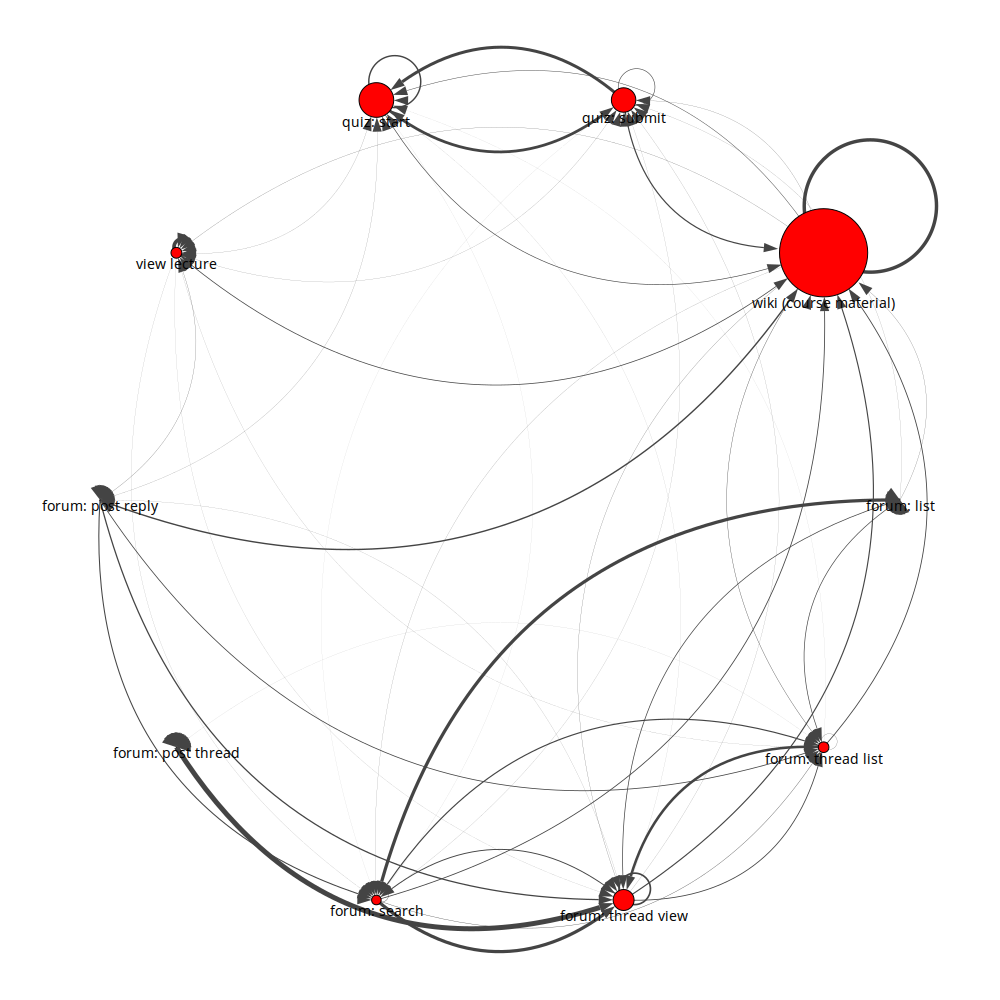
\includegraphics[width=\textwidth]{figures/text-6state/state0.png}
    \caption{An example ``quiz taking'' state.}
    \label{fig:practice-quiz-state}
  \end{subfigure}%
  \begin{subfigure}[t]{0.5\textwidth}
    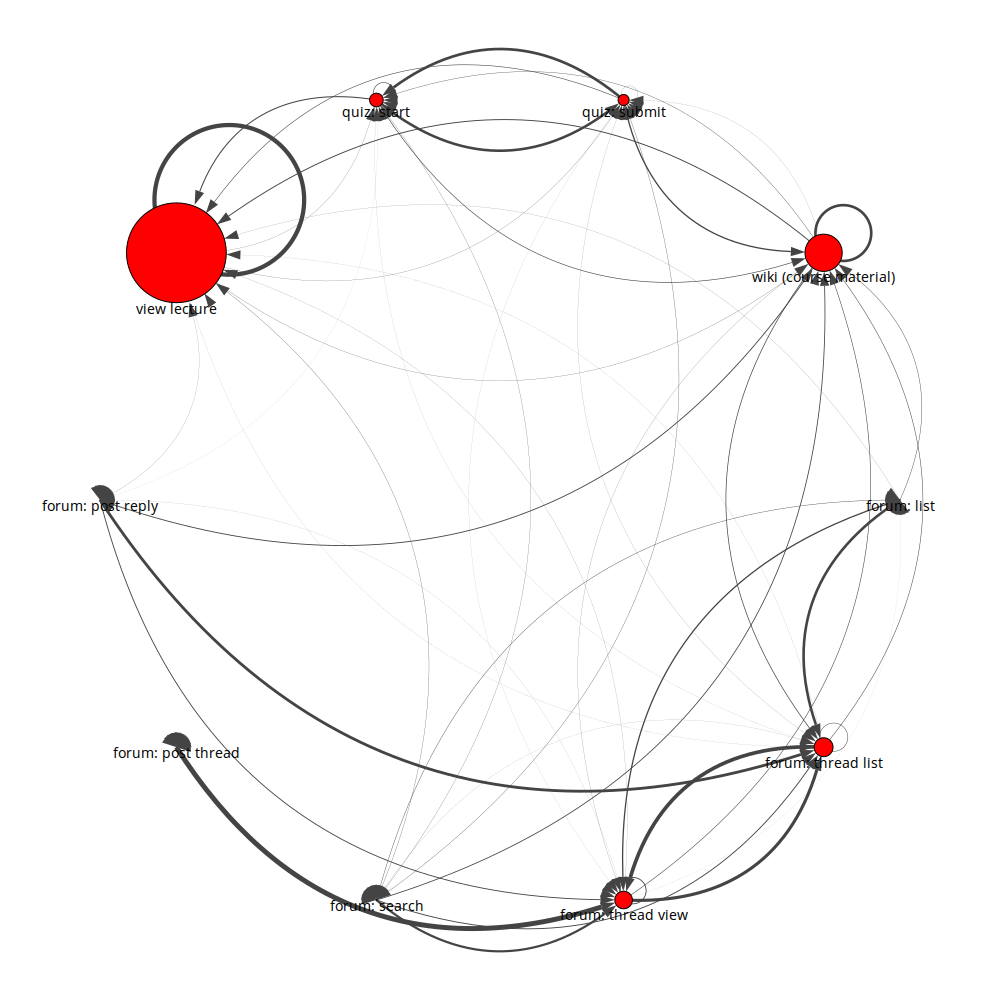
\includegraphics[width=\textwidth]{figures/text-6state/state1.png}
    \caption{An example ``lecture viewing'' state.}
    \label{fig:lecture-viewing-state}
  \end{subfigure}
  \caption{Two example states found by the 6-state TL-HMM.}
  \label{fig:states}
\end{figure*}

Figure~\ref{fig:states} includes two such representations we learned. The
first corresponds to a ``quiz taking'' state whereas the second corresponds
to a ``lecture viewing'' state. Clearly, our unsupervised method can
uncover states that do indeed correspond to student behavior modes that we
would expect to find a priori.

We also argue that it is important that the latent state representation be
a Markov model rather than just a discrete distribution over actions in
$\mathbf{A}$ (as would be the case for a traditional single-layer HMM). We
can observe why if we take a closer look at each of the two latent state
representations in Figure~\ref{fig:states} and look at their forum
component (bottom right). We can see that the relative probability of the
forum activities is roughly the same between these states, but the
\emph{transitions} are quite different. In
Figure~\ref{fig:practice-quiz-state} we have a relatively low probability
of walking from the ``forum thread view'' action back to the ``forum thread
list'' action, but in Figure~\ref{fig:lecture-viewing-state} we actually
observe a very strong link in this direction. This difference highlights an
important distinction between these two latent states: in the first you are
more likely to visit the forum \emph{looking for a particular post}, where
in the second you are more likely to visit the forum \emph{to browse
existing posts}. Thus, capturing the action transition matrix within a
latent state is important for capturing detailed insights involving bigrams
of actions.

\begin{figure*}
  \centering
  \begin{subfigure}[t]{0.5\textwidth}
    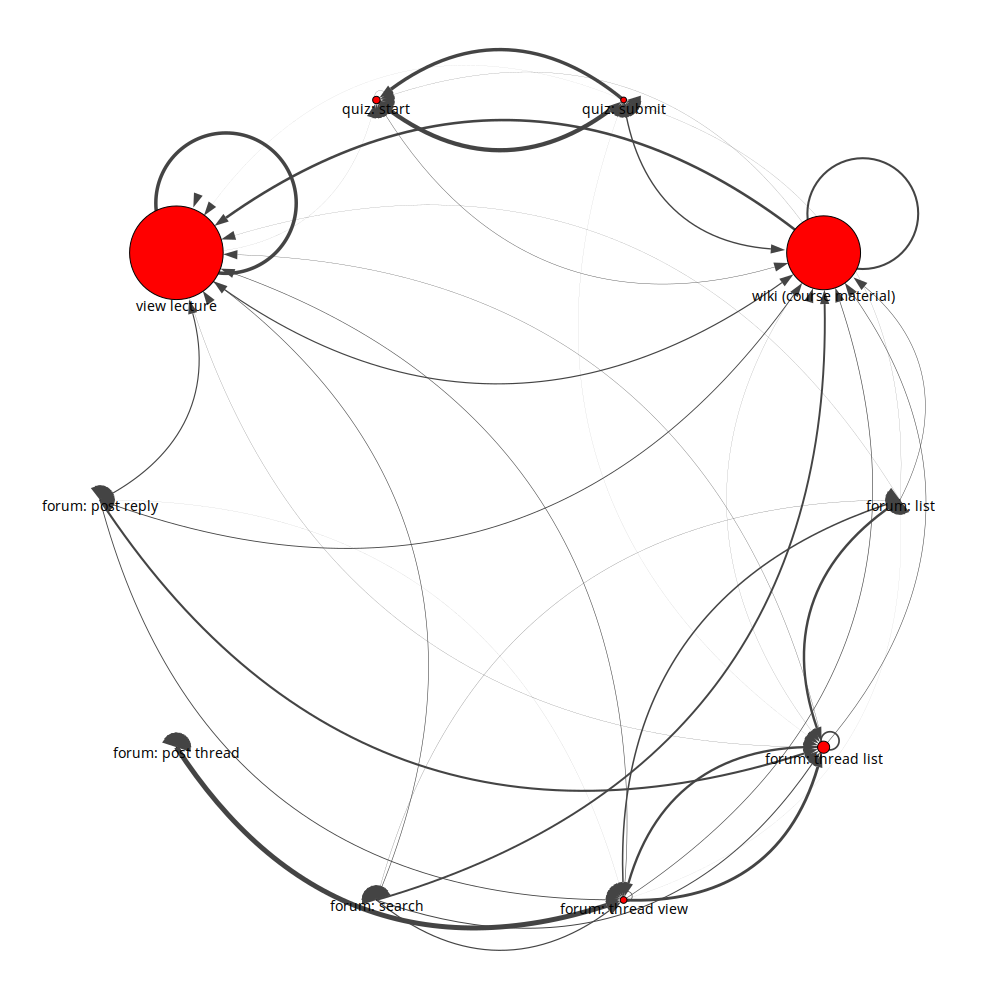
\includegraphics[width=\textwidth]{figures/text-6state/state4.png}
    \caption{A state from \textretrieval{}.}
  \end{subfigure}%
  \begin{subfigure}[t]{0.5\textwidth}
    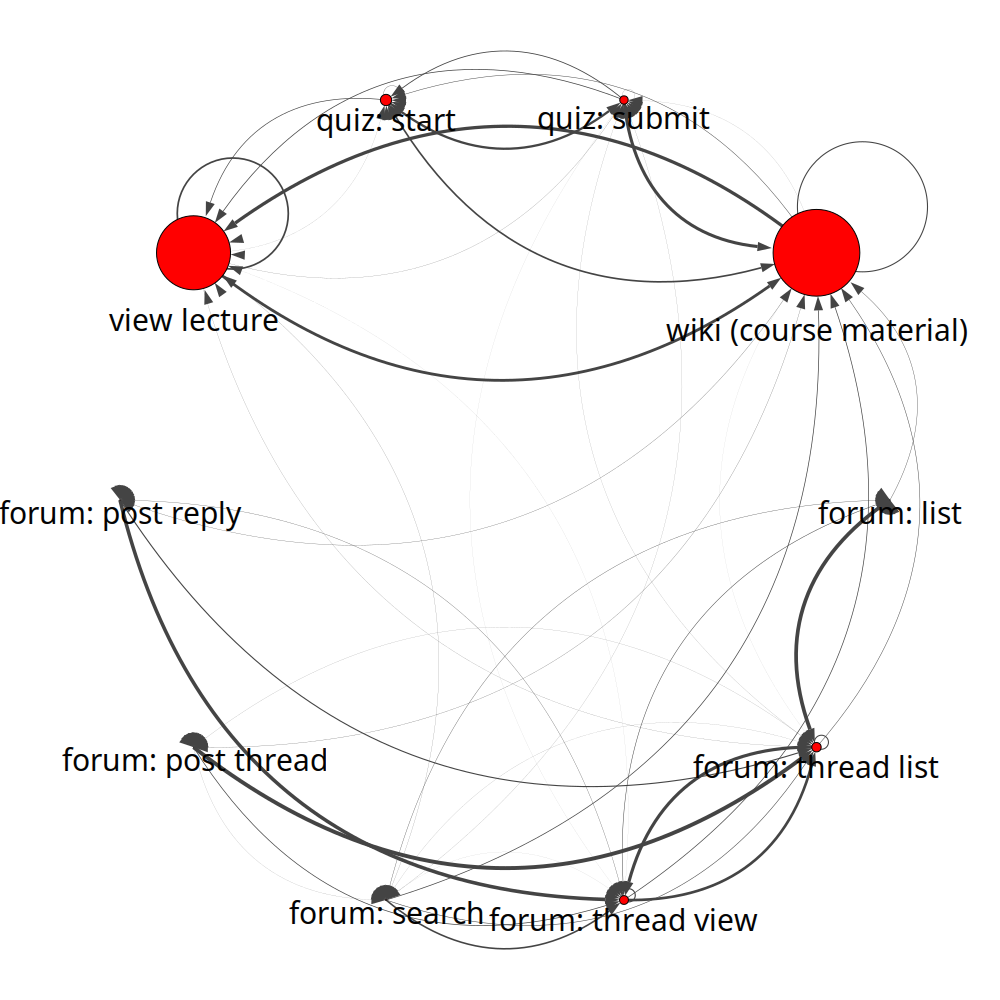
\includegraphics[width=\textwidth]{figures/sustain-6state/state4.png}
    \caption{A state from \sustain{}.}
  \end{subfigure}
  \caption{Two similar example states found by the 6-state TL-HMM.}
  \label{fig:cross-course}
\end{figure*}

We can also use our model for cross-course behavior analysis. In
Figure~\ref{fig:cross-course} we show two latent state representations
learned by a 6-state TL-HMM, one from \textretrieval{} and one from
\sustain{}. These two states were chosen as they are the most similar
across the two courses. However, if we look at the transitions we can see
some important differences. First, in the state from \textretrieval{}, we
can see that the probability of returning to the course wiki after viewing
a lecture is considerably lower than that probability in the state from
\sustain{}. We also notice that the self-loop for staying in a lecture
activity in \textretrieval{} is significantly higher probability than it is
in the state from \sustain{}. This gives us some insight into the lecture
viewing behavior of students in these two MOOCs which can possibly be a
reflection of the course's structure. In \textretrieval{}, students are
likely to view lecture videos in succession directly without first visiting
the course wiki, whereas in \sustain{} students are much more likely to
first return the course wiki before watching the next lecture video. This
observation would be lost if we did not consider the transitions between
the actions within the latent states.

\subsection{Varying the Number of Latent States}
Our TL-HMM model has a parameter $K$ that sets the number of latent states
to be learned. We believe that this can allow our model to flexibly
discover patterns of different granularity, and we can show this by varying
$K$ for a particular course and observing how the latent state
representations evolve.

\begin{figure*}
  \centering
  \begin{tabular}{cccc}
    \textbf{State 0} & \textbf{State 1} & \textbf{State 2} & \textbf{State
    3}\\\hline
    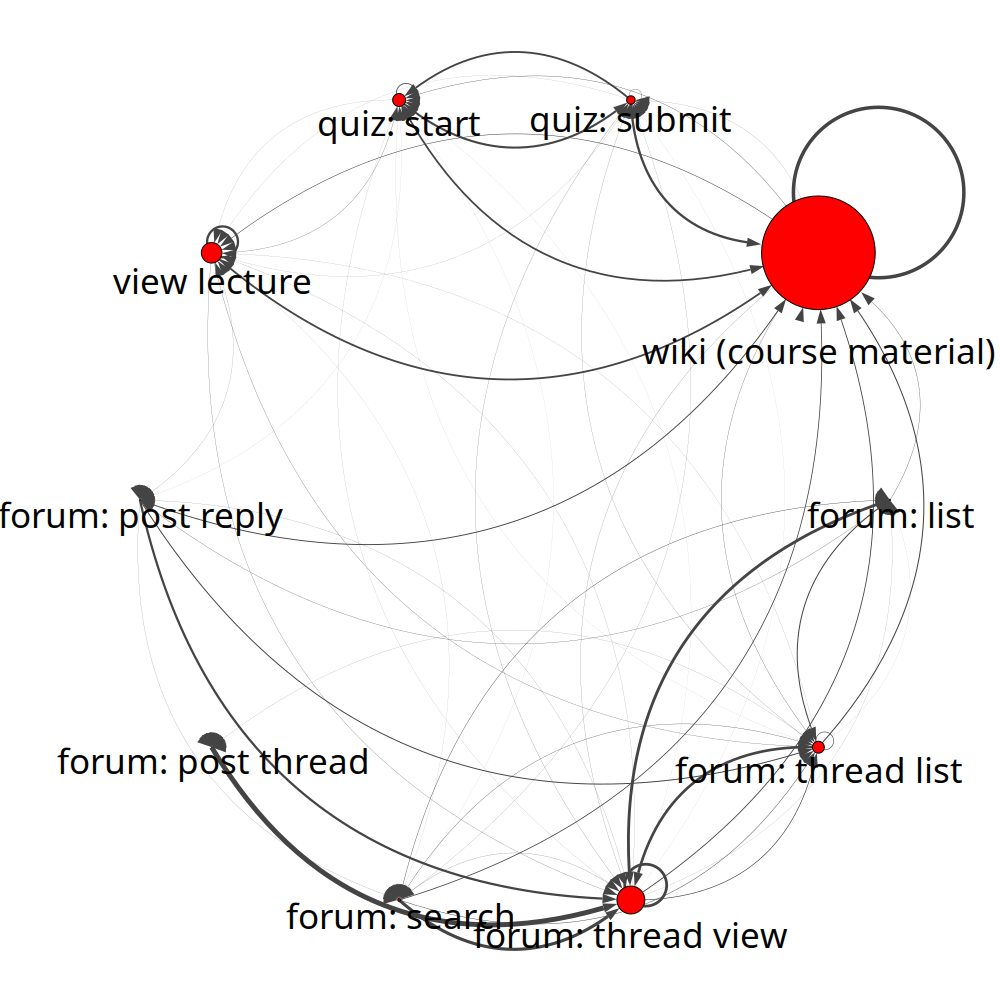
\includegraphics[width=0.22\textwidth]{figures/text-2state/state0.png}
    &
    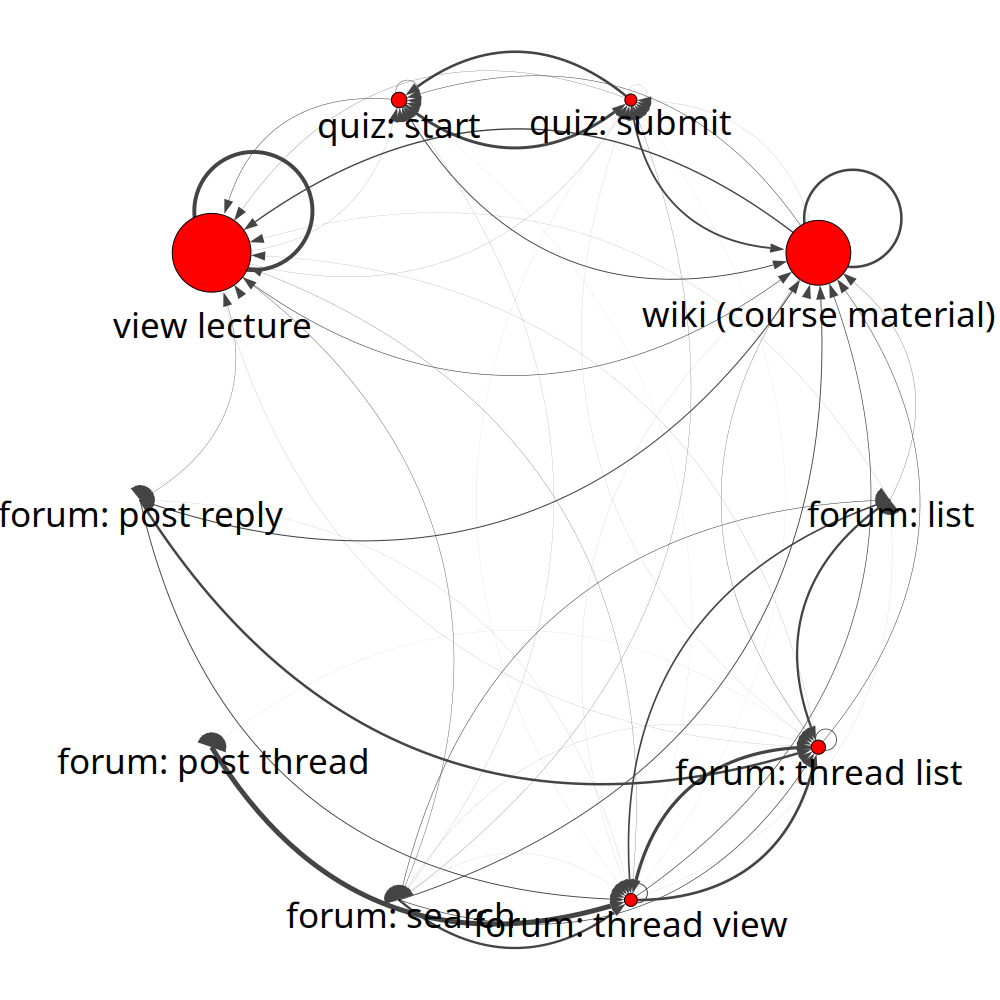
\includegraphics[width=0.22\textwidth]{figures/text-2state/state1.png}\\
    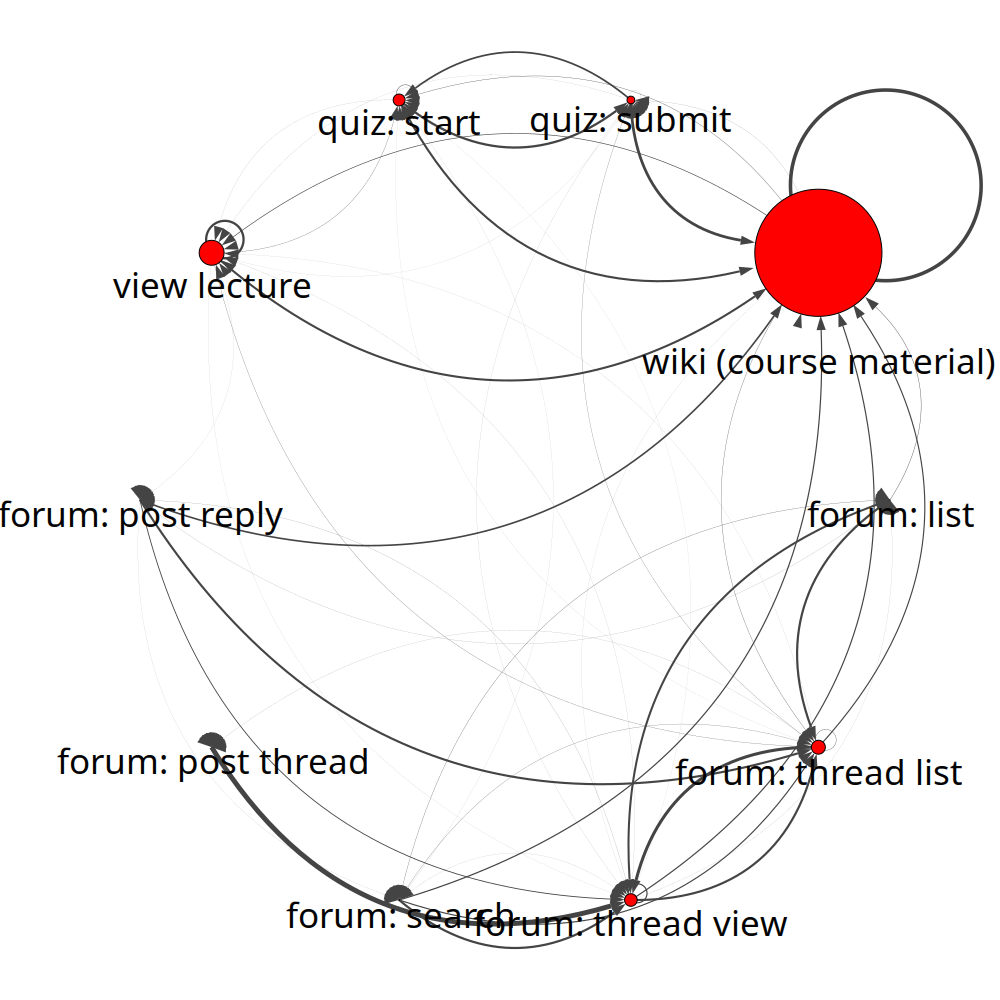
\includegraphics[width=0.22\textwidth]{figures/text-3state/state0.png}
    &
    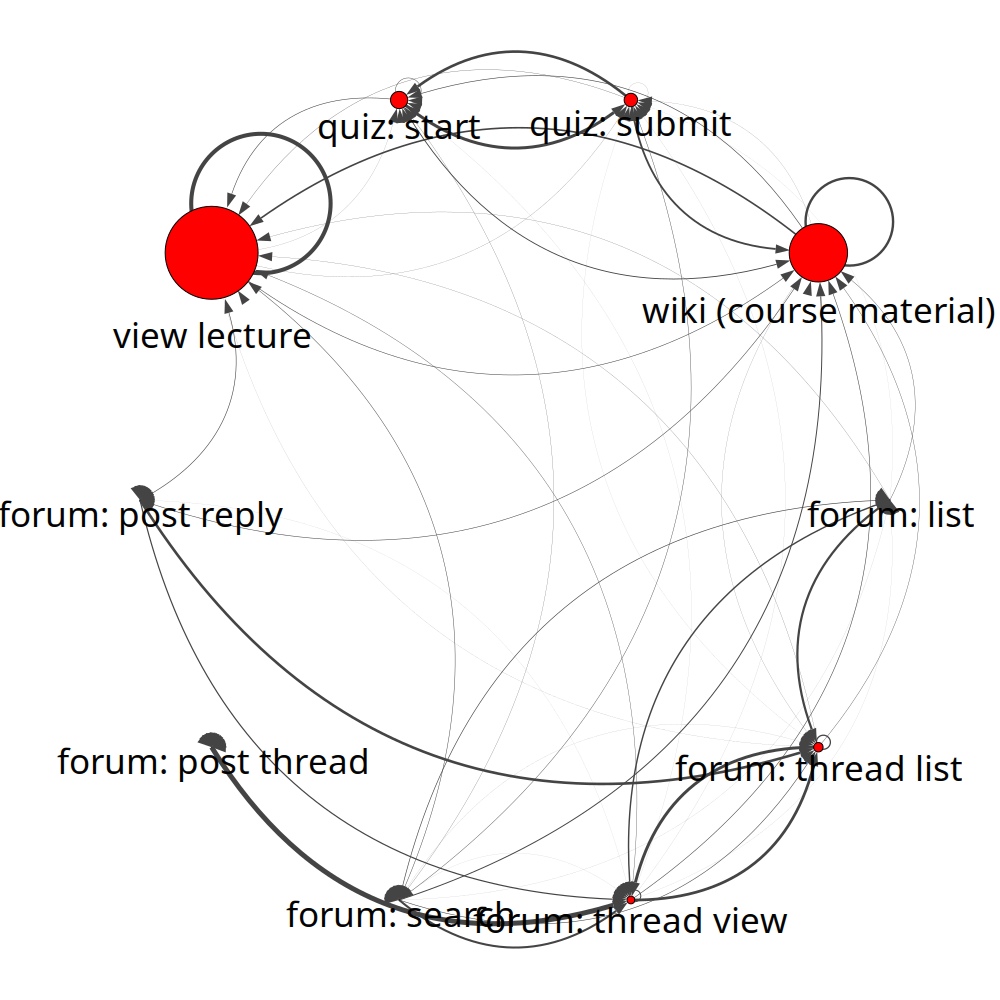
\includegraphics[width=0.22\textwidth]{figures/text-3state/state1.png}
    &
    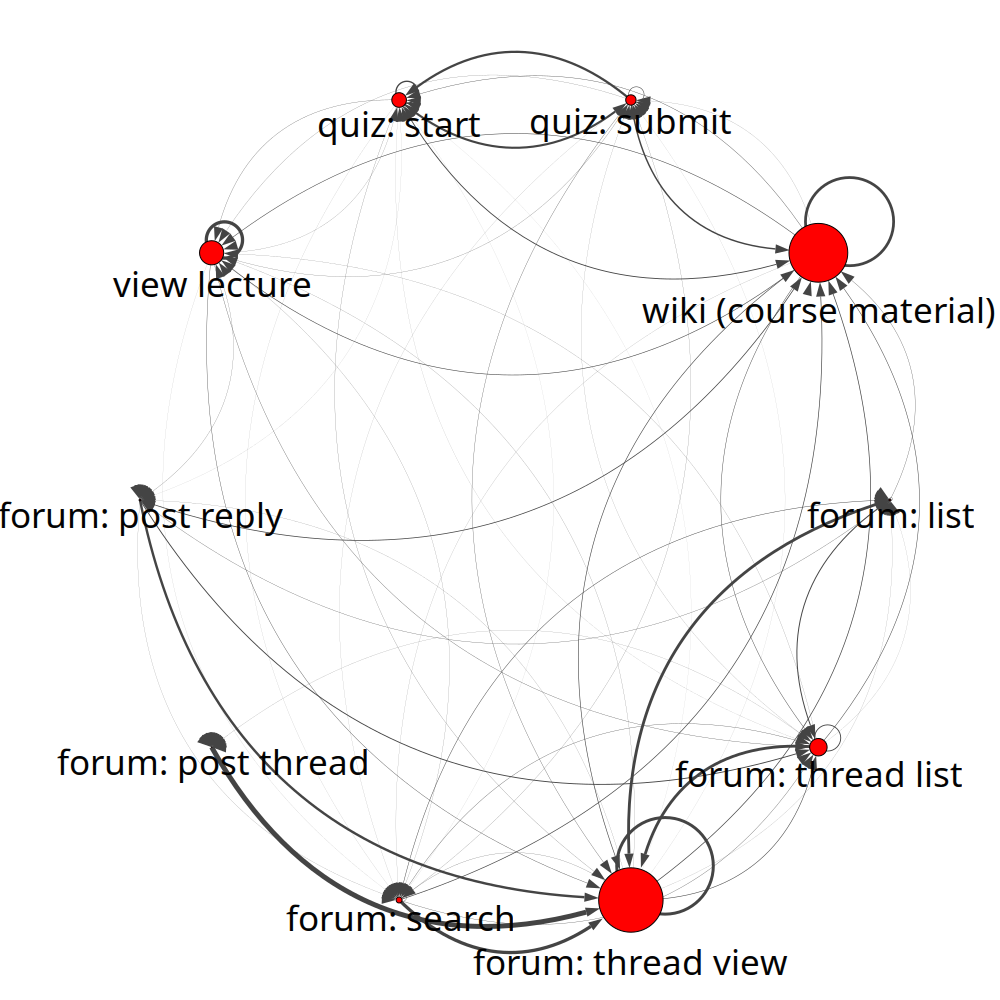
\includegraphics[width=0.22\textwidth]{figures/text-3state/state2.png}\\
    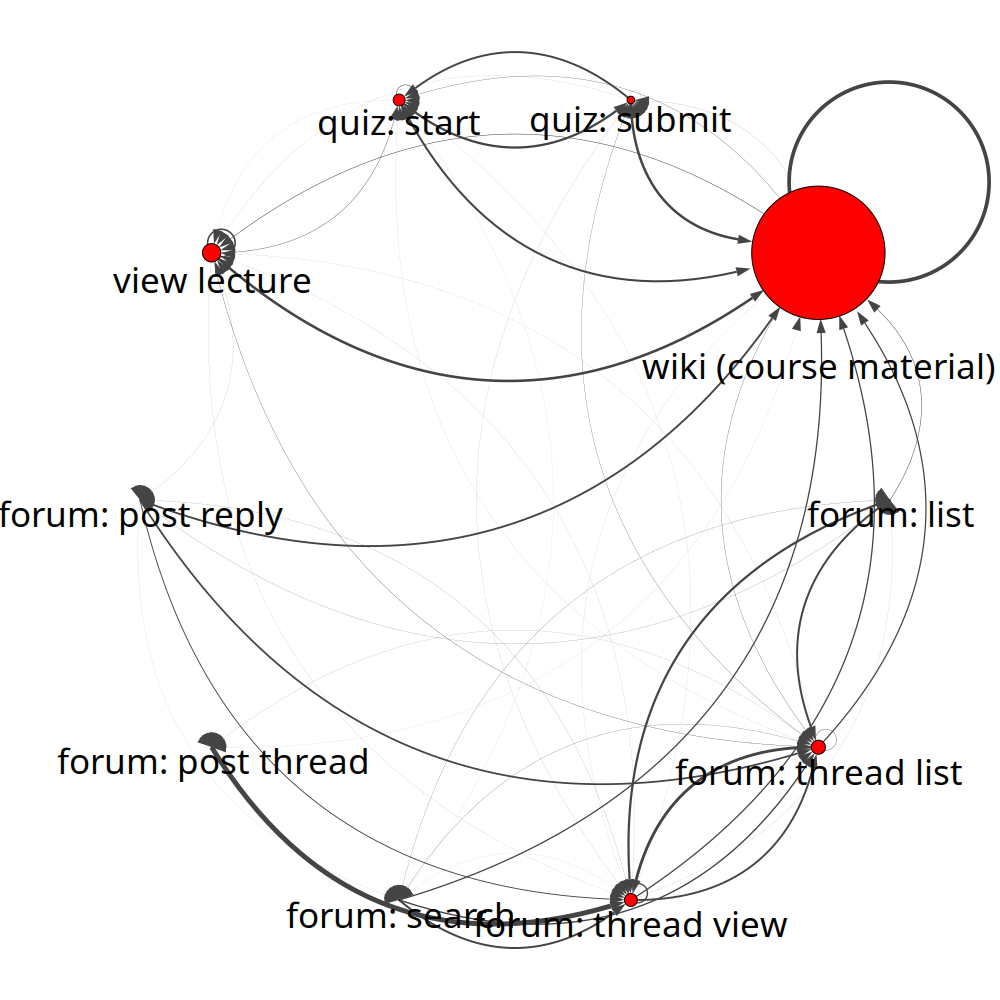
\includegraphics[width=0.22\textwidth]{figures/text-4state/state0.png}
    &
    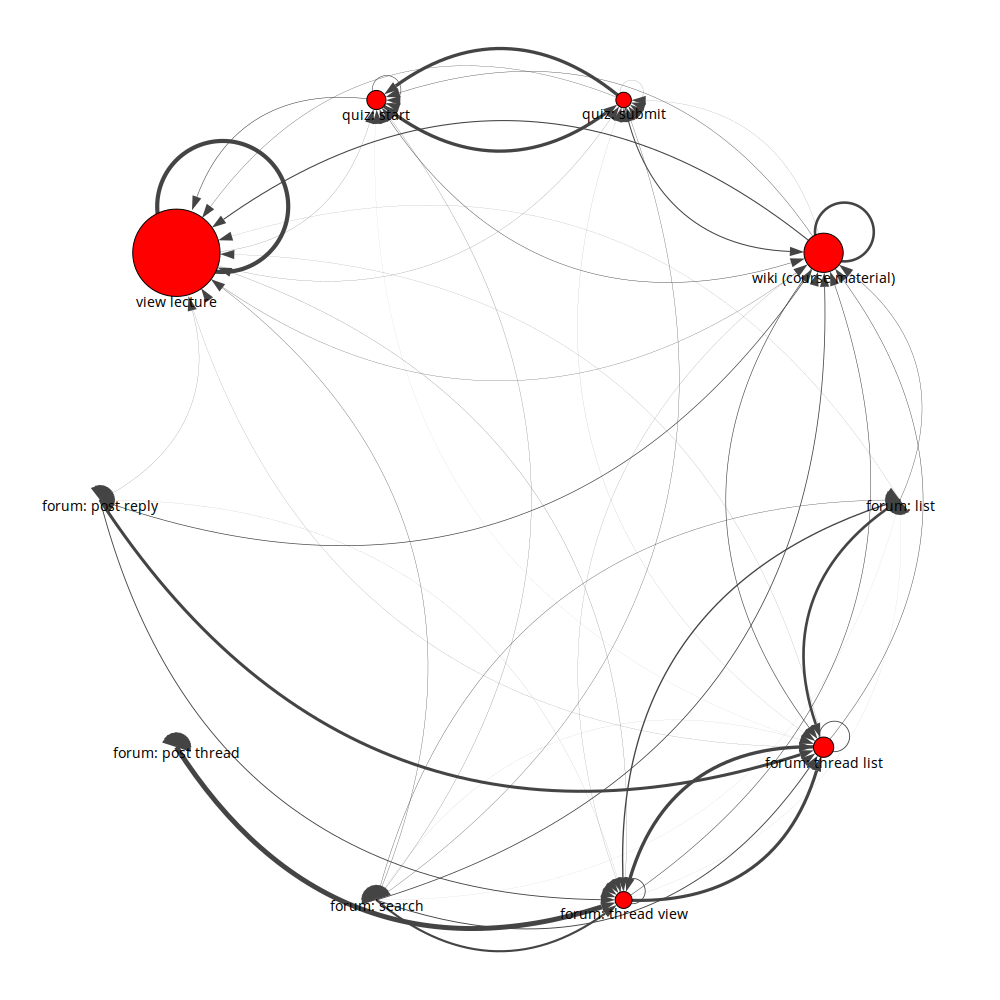
\includegraphics[width=0.22\textwidth]{figures/text-4state/state1.png}
    &
    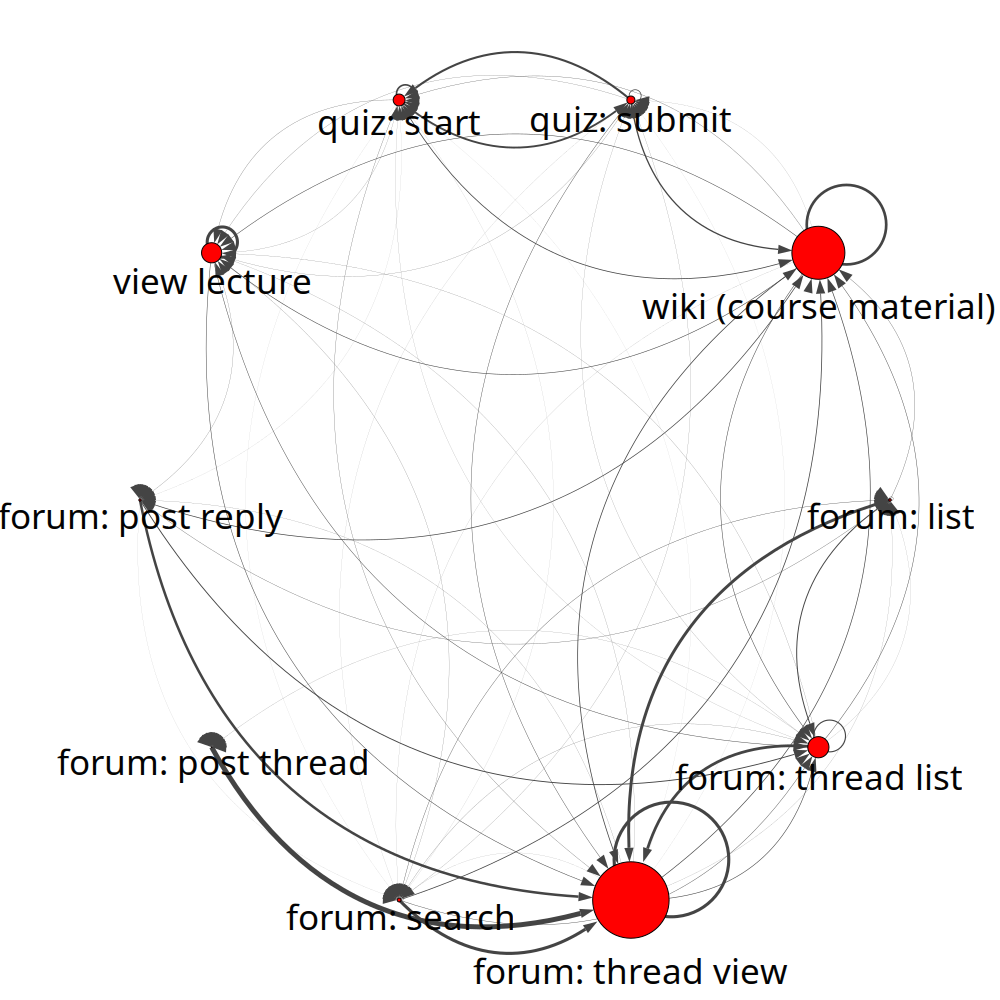
\includegraphics[width=0.22\textwidth]{figures/text-4state/state2.png}
    &
    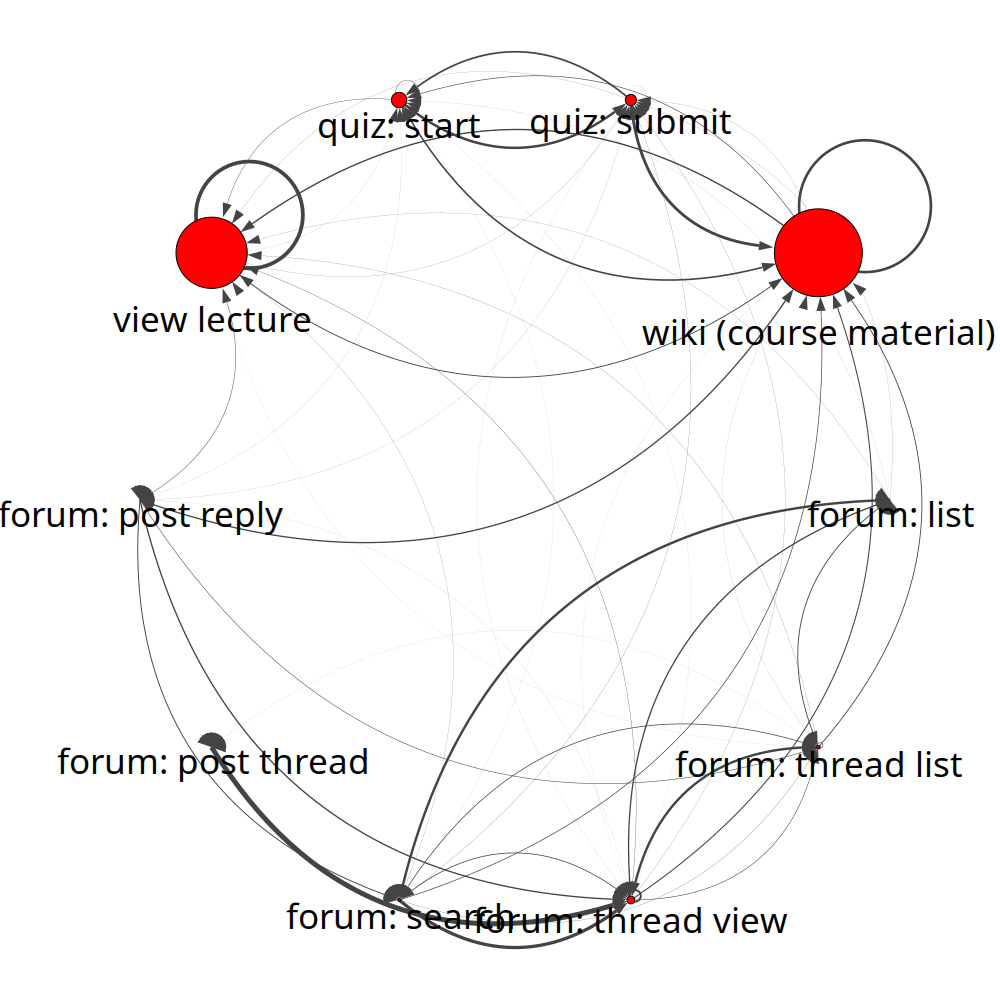
\includegraphics[width=0.22\textwidth]{figures/text-4state/state3.png}
  \end{tabular}
  \caption{The evolution of states for increasing $K$ for the
  \protect\textretrieval{} MOOC.} % I don't know why \protect is needed
  \label{fig:text-state-evolution}
\end{figure*}

In Figure~\ref{fig:text-state-evolution} we see the evolution of the latent
state representations found for the \textretrieval{} MOOC\footnote{Due to
space constraints, the graphs are quite small, but the states are in the
same positions as they were in previous figures to aid interpretation.}.
With $K=2$ we uncover a video watching pattern (state 1) and a course
material browsing pattern (state 0). However, we can see that when $K=3$ we
are able to uncover a new pattern involving forum behavior in state 3
(notice the node sizes on the bottom right). As we increase $K$ to four, we
can see that state 1 splits into state 1 and state 3. These states appear
quite similar at a glance, but there are still some key differences. First,
we can see that state 1 now has a non-negligible forum component, whereas
state 3 has hardly any weight on the forum.

\begin{figure*}
  \centering
  \begin{tabular}{cccc}
    \textbf{State 0} & \textbf{State 1} & \textbf{State 2} & \textbf{State
    3}\\\hline
    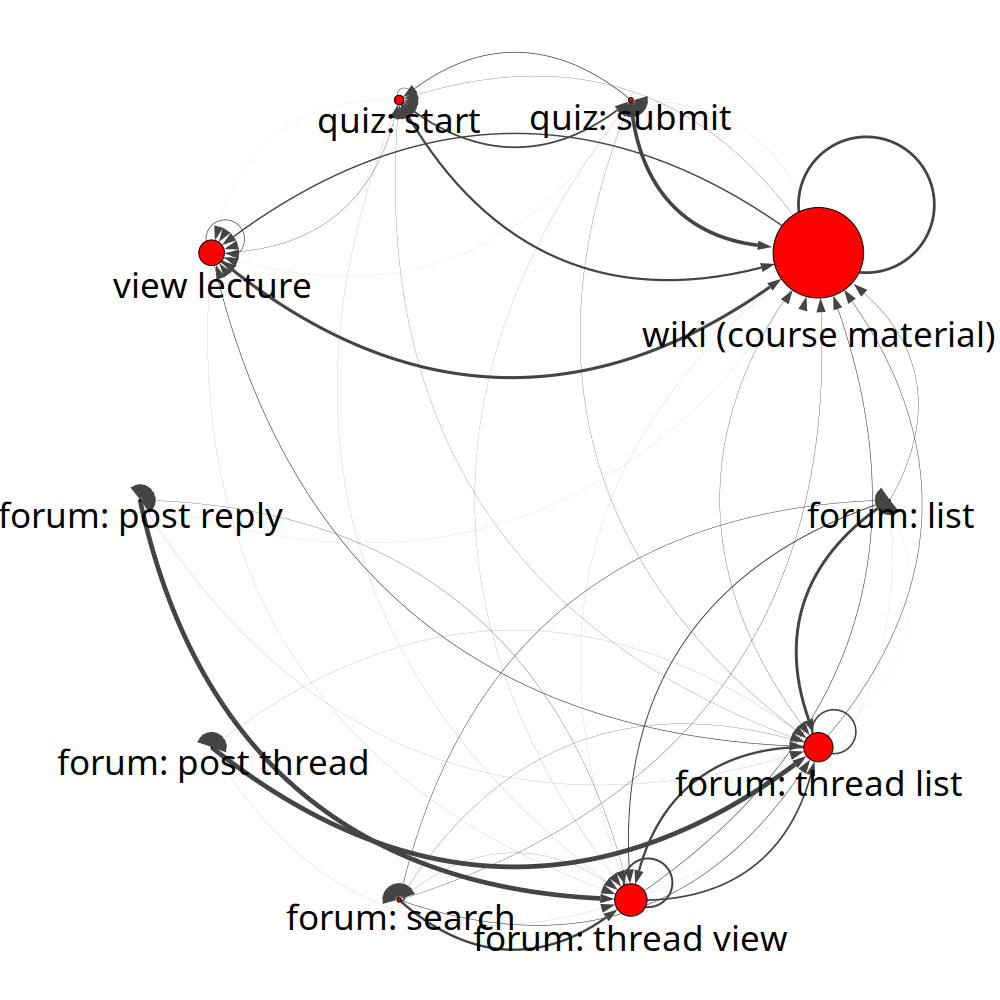
\includegraphics[width=0.22\textwidth]{figures/sustain-2state/state0.png}
    &
    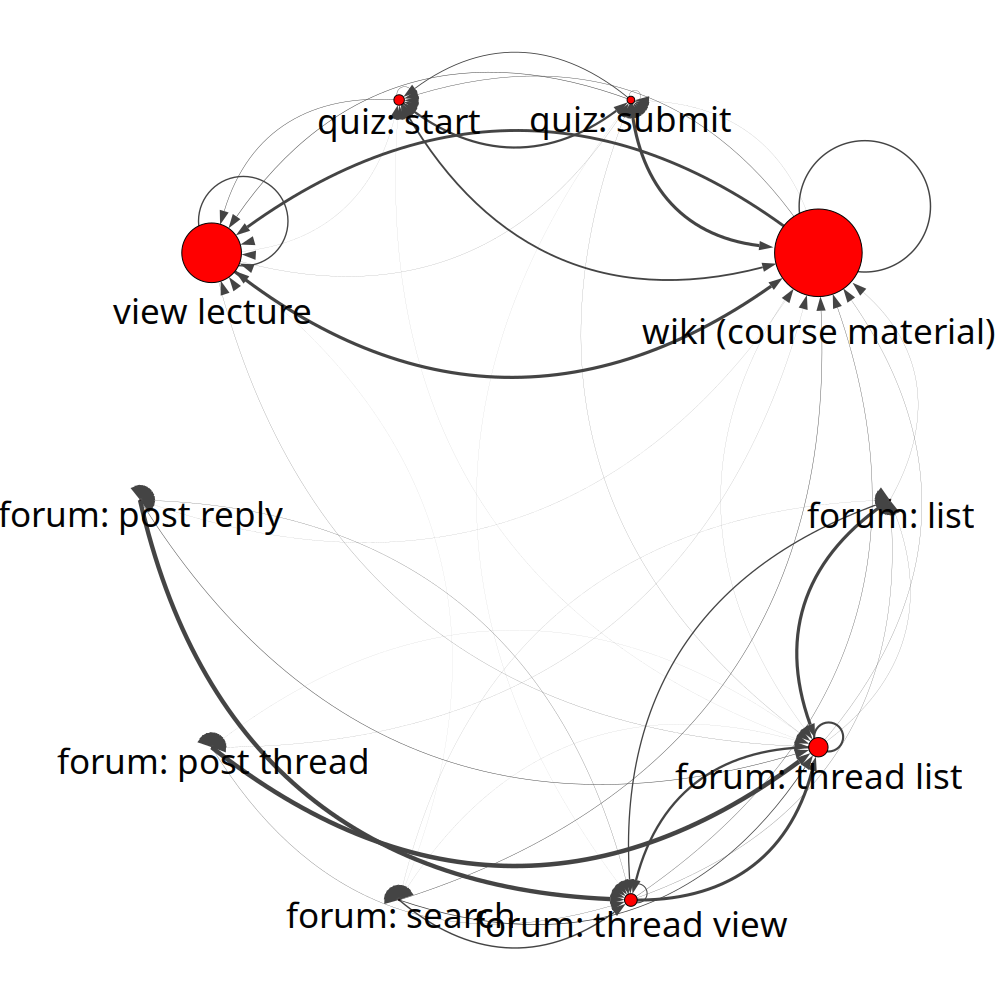
\includegraphics[width=0.22\textwidth]{figures/sustain-2state/state1.png}\\
    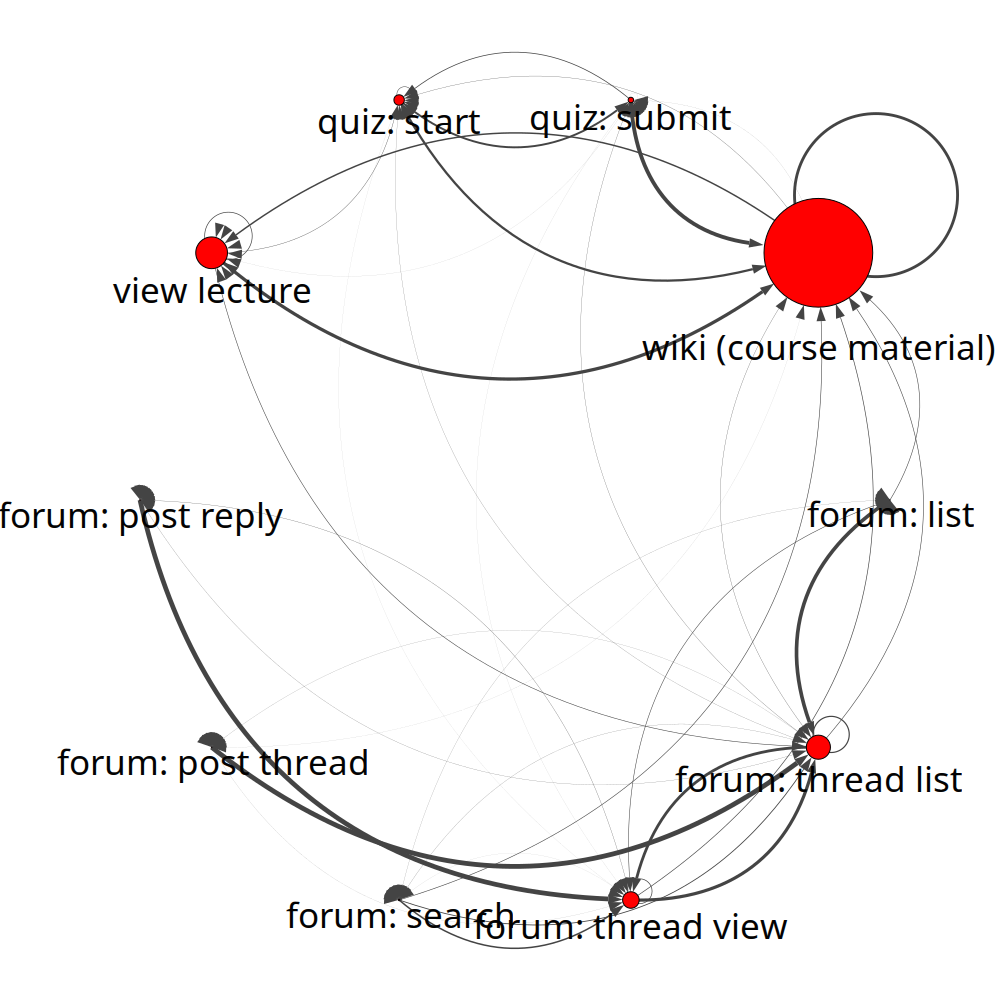
\includegraphics[width=0.22\textwidth]{figures/sustain-3state/state0.png}
    &
    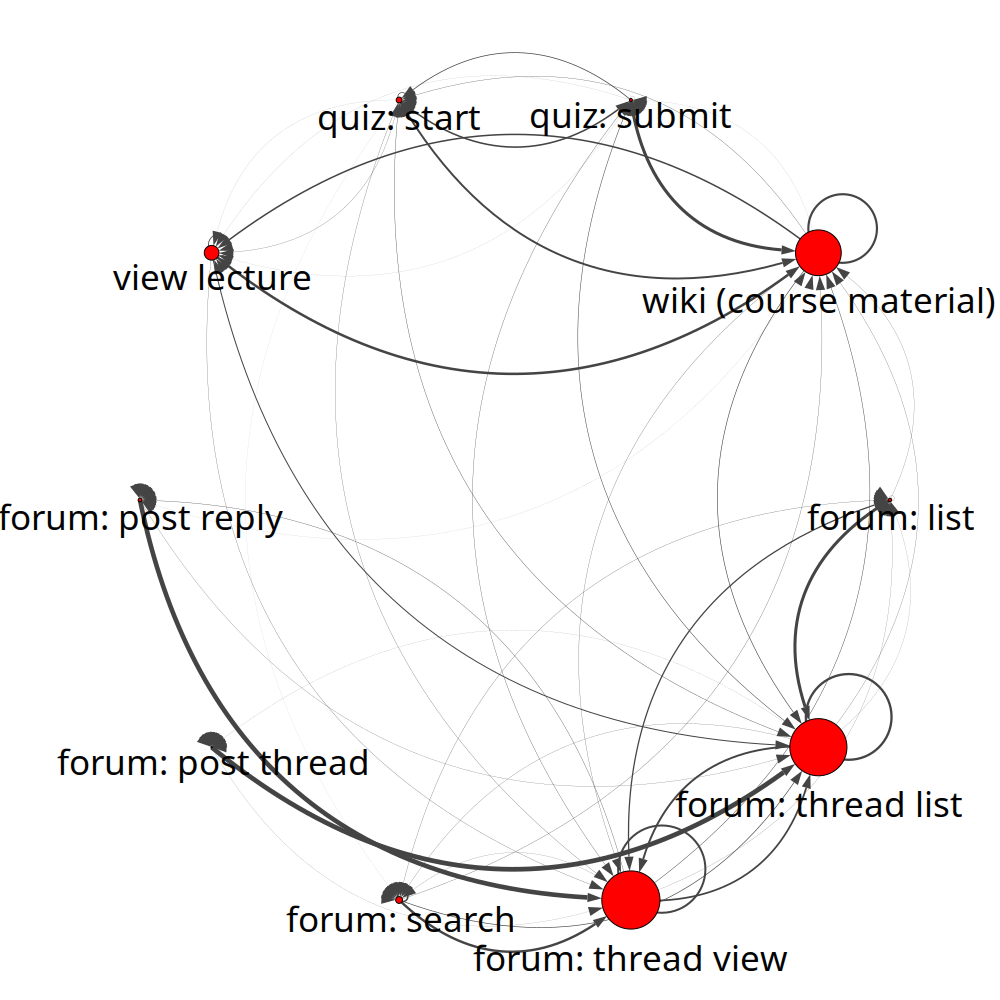
\includegraphics[width=0.22\textwidth]{figures/sustain-3state/state1.png}
    &
    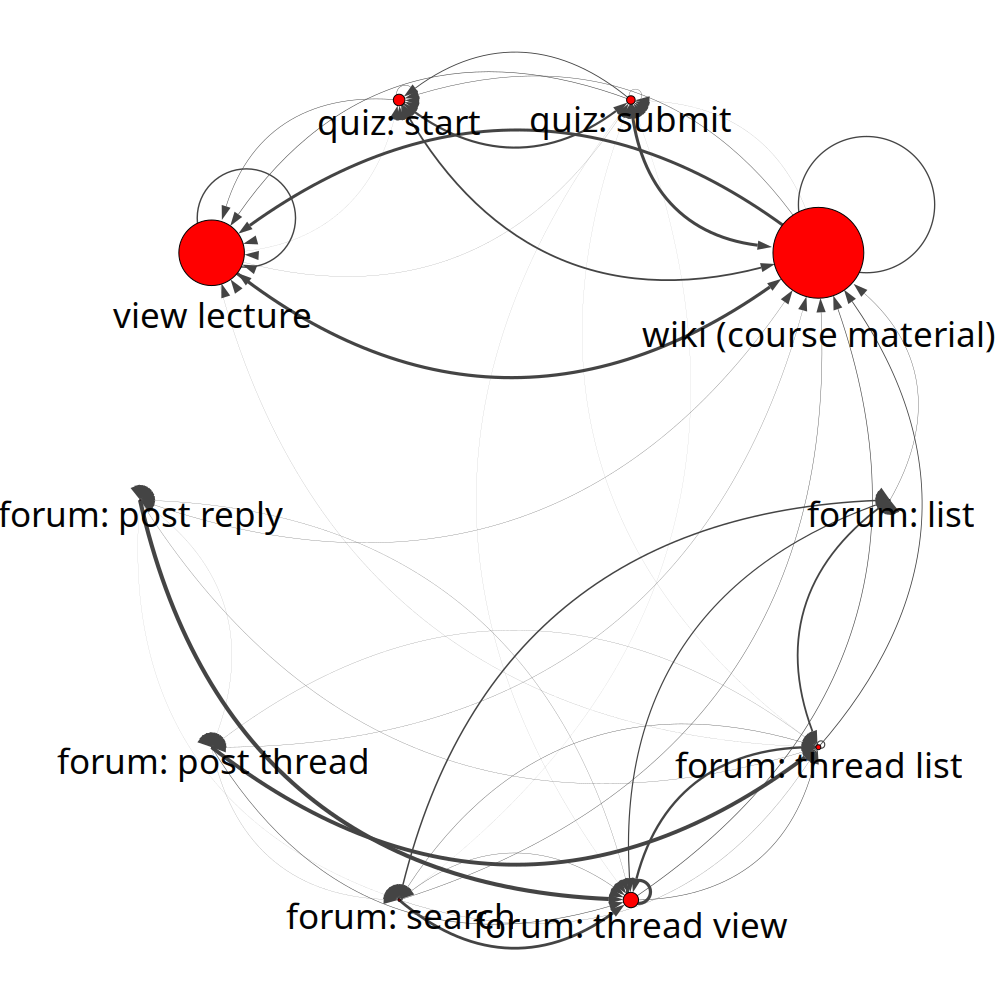
\includegraphics[width=0.22\textwidth]{figures/sustain-3state/state2.png}\\
    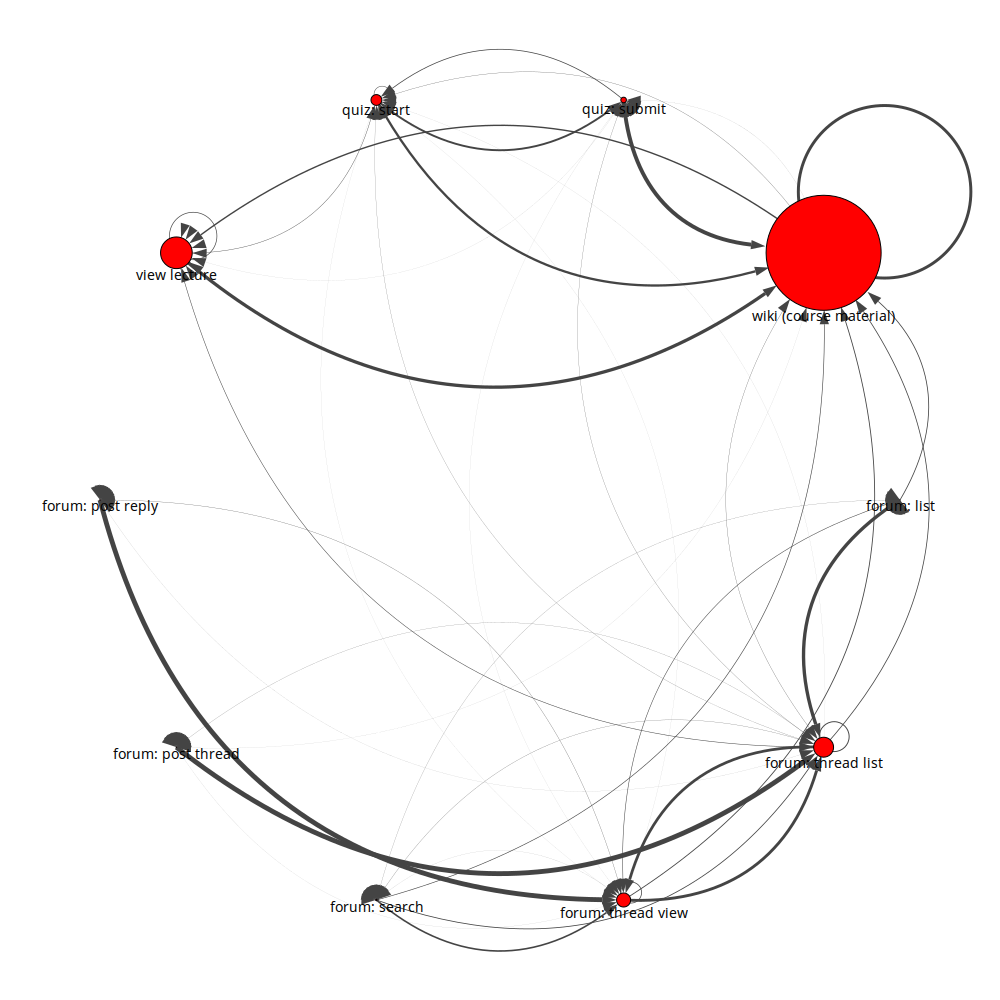
\includegraphics[width=0.22\textwidth]{figures/sustain-4state/state0.png}
    &
    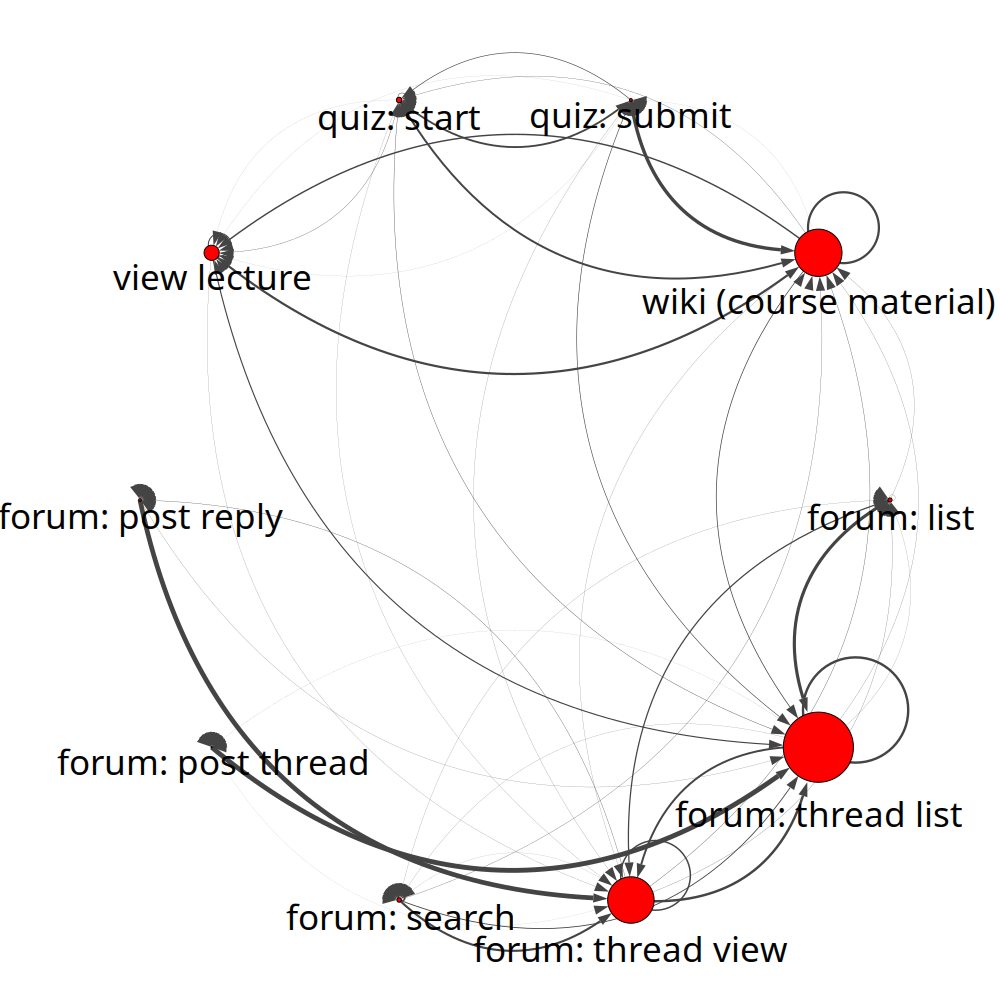
\includegraphics[width=0.22\textwidth]{figures/sustain-4state/state1.png}
    &
    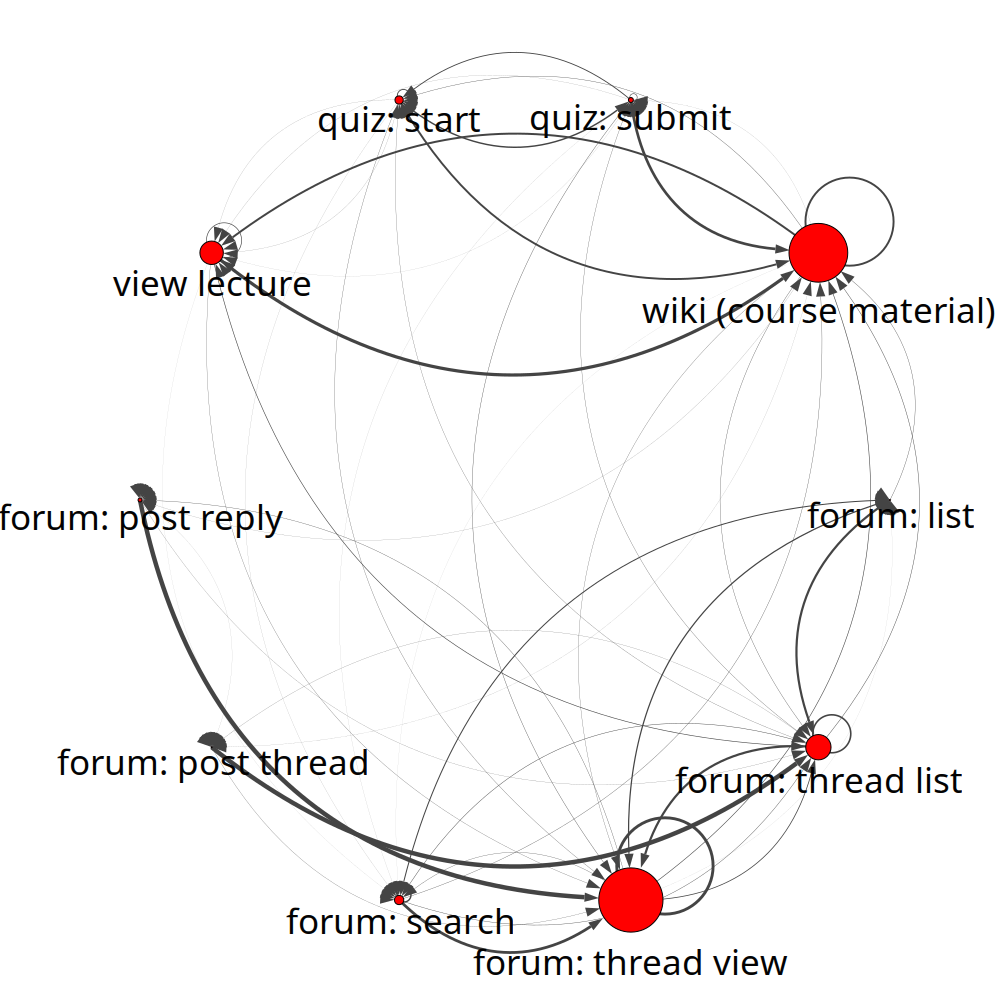
\includegraphics[width=0.22\textwidth]{figures/sustain-4state/state2.png}
    &
    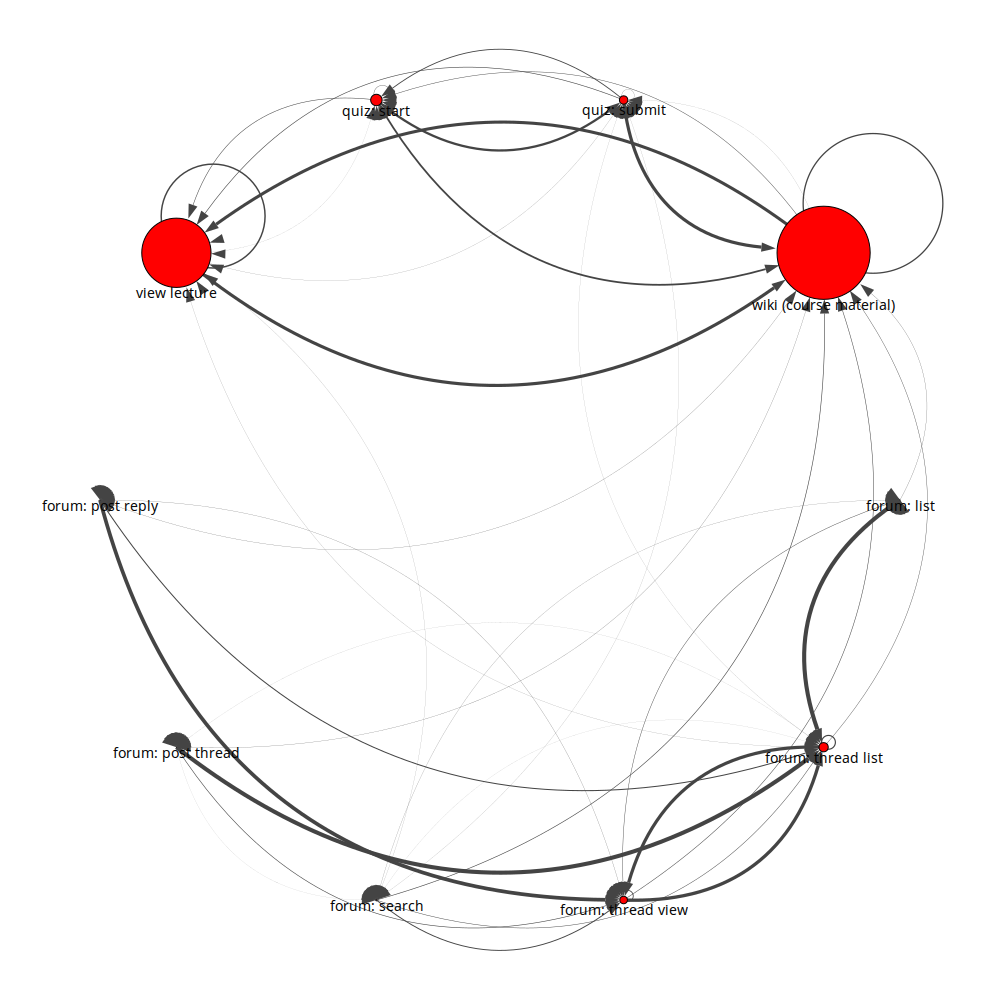
\includegraphics[width=0.22\textwidth]{figures/sustain-4state/state3.png}
  \end{tabular}
  \caption{The evolution of states for increasing $K$ for the
  \protect\sustain{} MOOC.} % I don't know why \protect is needed
  \label{fig:sustain-state-evolution}
\end{figure*}

We observe similar behavior in Figure~\ref{fig:sustain-state-evolution}
as we increase $K$ when fitting our TL-HMM on the \sustain{} MOOC. Again,
in the transition between $K=2$ and $K=3$ we discover forum behavior
patterns as a latent state. However, in the transition between $K=3$ to
$K=4$ we instead see a refining of that discovered forum state, where
state 2 captures asymmetric transition probabilities between ``forum thread
view'' and ``forum thread list''. These states could be seen as redundant,
in which case a more appropriate setting of $K=3$ may be appropriate for
the \sustain{} dataset.

\subsection{Transitions Between Latent States}

\begin{figure*}
  \centering
  \begin{subfigure}[t]{0.5\textwidth}
    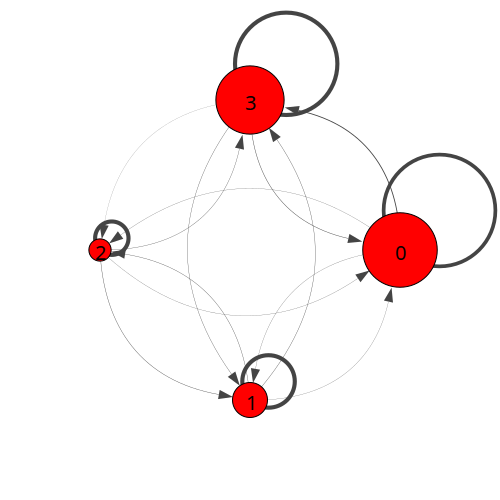
\includegraphics[width=\textwidth,trim={0 3cm 0 2cm}]{figures/trans-comp/trans-avg.png}
    \caption{\label{fig:trans-avg}}
  \end{subfigure}%
  \begin{subfigure}[t]{0.5\textwidth}
    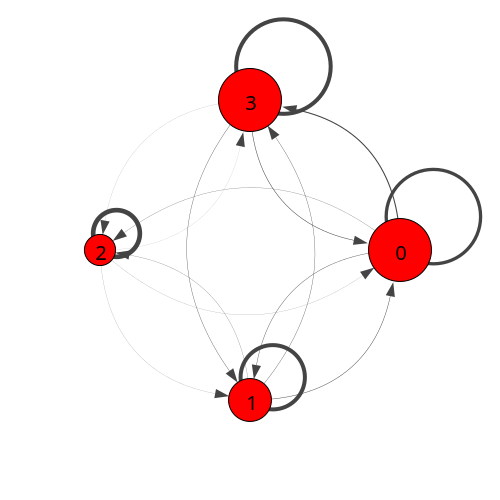
\includegraphics[width=\textwidth,trim={0, 3cm 0 2cm}]{figures/trans-comp/trans-perfect.png}
    \caption{\label{fig:trans-perfect}}
  \end{subfigure}
  \caption{The latent state transition diagrams for a 4-state TL-HMM fit to
  \protect\textretrieval{} for all students (a) compared to only ``perfect''
  students (b).}
  \label{fig:trans-comp}
\end{figure*}

A unique property of our model is its ability to capture transitions
between the \emph{behavior patterns themselves} that are captured by the
latent states. In Figure~\ref{fig:trans-avg} we show the latent state
transition diagram for a 3-state TL-HMM fit on \textretrieval{}. We can
immediately observe two things: \begin{enumerate*}[label=(\arabic*)]
  \item each latent state has a very high ``staying'' probability, and
  \item the prevalence of each latent state matches our intuition.
\end{enumerate*}
In particular, we can see that the forum browsing state (state 2) has
relatively lower probability than the other states as we might expect. It
also makes sense that state 0 has rather high probability as this state
likely captures all sequences where a student logged in to the platform and
then did nothing else (likely checking for updates). If we look at state 1
and state 3, their relative probabilities match our intuition as
well. State 1 seems to capture a more engaged browsing session, where there
is non-negligible probability associated with different activities such as
quiz taking and forum browsing and, importantly, these activities have high
probability symmetric edges (so students are taking quizzes one after the
other, or viewing forum threads in succession). By contrast, state 3 seems
to capture a more passive student, with negligible probability mass
associated with forum activity (with low symmetry in the edges). The link
between ``quiz submit'' and ``quiz start'' (indicating quiz repetition) is
also significantly lower than state 1.

Thus, we might expect to see students that perform well in the course
preferring states 1 and 2 over states 0 and 3. To verify this, we took the
model we learned on the full training data and retrofit it to training data
consisting only of sequences produced by students in \textretrieval{} that
had perfect marks. To prevent the latent state meanings from drifting, we
forced the model parameters associated with their Markov model
representations to be fixed, in effect only learning initial and transition
probabilities for the top layer of our TL-HMM.\ We show the updated latent
state transition diagram in Figure~\ref{fig:trans-perfect}. We can clearly
see that the probability of state 2 has increased dramatically, while the
probability of states 0 and 3 has decreased. State 1 had its probability
increase, but only very slightly.
